\documentclass[a4paper,12pt]{article}
\usepackage[latin1]{inputenc}
\usepackage[spanish]{babel}
\usepackage{calc, graphicx}
\usepackage[format=hang, font=small, labelfont=bf, labelsep=endash, width=.9\textwidth]{caption}
\usepackage[listofformat=subsimple, format=hang, labelfont=footnotesize, textfont={it, footnotesize}]{subfig}
\title{Figuras elaboradas con MetaPost}
\author{Jos� Ram�n Gisbert Valls}
\newcommand\texto{Este manual est� destinado a todo aquel usuario interesado en la representaci�n de se�ales el�ctricas en el contexto que se ha expuesto anteriormente en el libro. En concreto, puede ser de especial inter�s para aquellos usuarios que deseen representar el espectro en frecuencia de una se�al el�ctrica en tiempo real, de forma que al mismo tiempo pueda visualizarse la se�al correspondiente a dicho espectro.}
\begin{document}


\maketitle{}

\begin{abstract}
	Este documento me permite seguir el aspecto que muestran las figuras elaboradas en MetaPost para su inclusi�n en la memoria al ritmo en el que las voy desarrollando.
\end{abstract}

\listoffigures

% \begin{figure}
% 	\begin{center}
% 		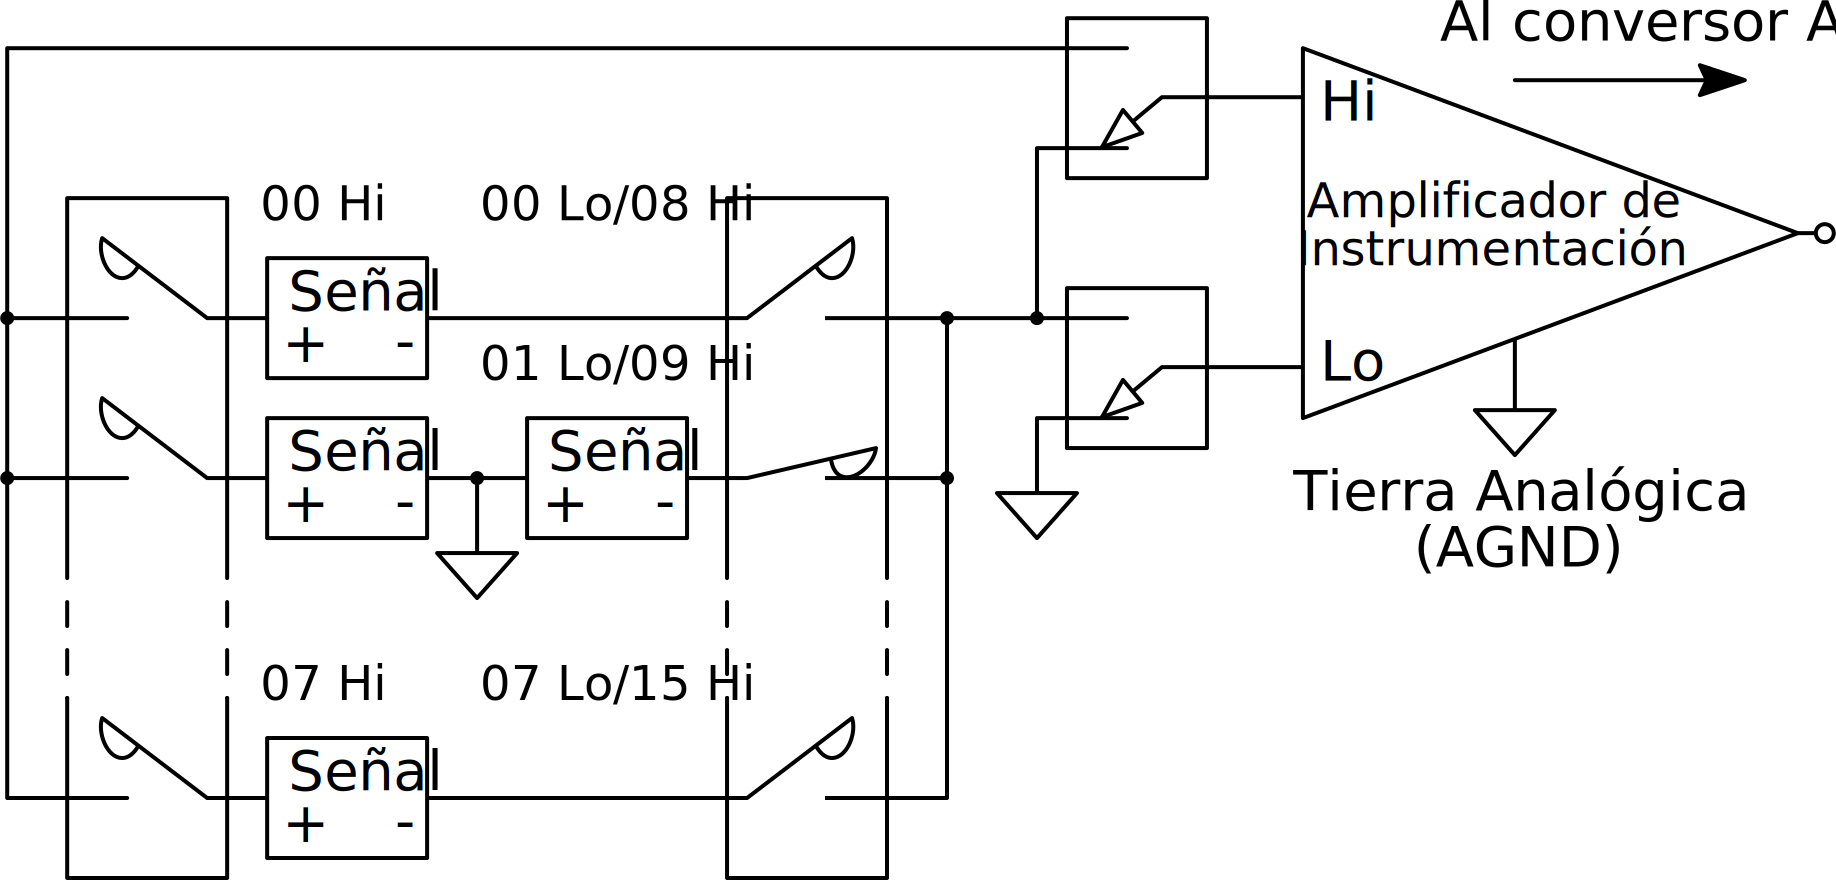
\includegraphics{gis-pfc-ch1-1.mps}
% 	\end{center}
% 	\caption[Ejemplo de configuraci�n de terminaci�n]{Figura que muestra el modo de terminaci�n sencillo. La entrada superior del amplificador de instrumentaci�n se conecta al puerto 9 y la entrada inferior se conecta a masa.}
% 	\label{fig:termmodes}
% \end{figure}
% 
\begin{figure}
	\begin{center}
		
\includegraphics{gis-pfc-ch2-2.mps}
	\end{center}
	\caption[Fragmento de se�al adquirido por el osciloscopio en el espacio de una ventana temporal]{Fragmento de se�al adquirido por el osciloscopio en el espacio de una ventana temporal. Puede apreciarse la informaci�n descartada y los cortes con el nivel de disparo, especialmente el corte central en el que se centrar� la representaci�n de la se�al.}
	\label{fig:freesignal}
\end{figure}

\begin{figure}
	\begin{center}
		\includegraphics{gis-pfc-ch2-3.mps}
	\end{center}
	\caption{Funcionamiento disparado del osciloscopio digital}
	\label{fig:digtrigosc}
\end{figure}
% 
% \begin{figure}
% 	\begin{center}
% 		\includegraphics{gis-pfc-ch2-4.mps}
% 	\end{center}
% 	\caption{Componentes de la \textsc{dat}.}
% 	\label{fig:dat}
% \end{figure}
% 
% \begin{figure}
% 	\begin{center}
% 		\includegraphics{gis-pfc-ch2-5.mps}
% 	\end{center}
% 	\caption{Tipos de objeto dispositivo.}
% 	\label{fig:devobject}
% \end{figure}
% 
% \begin{figure}
% 	\begin{center}
% 		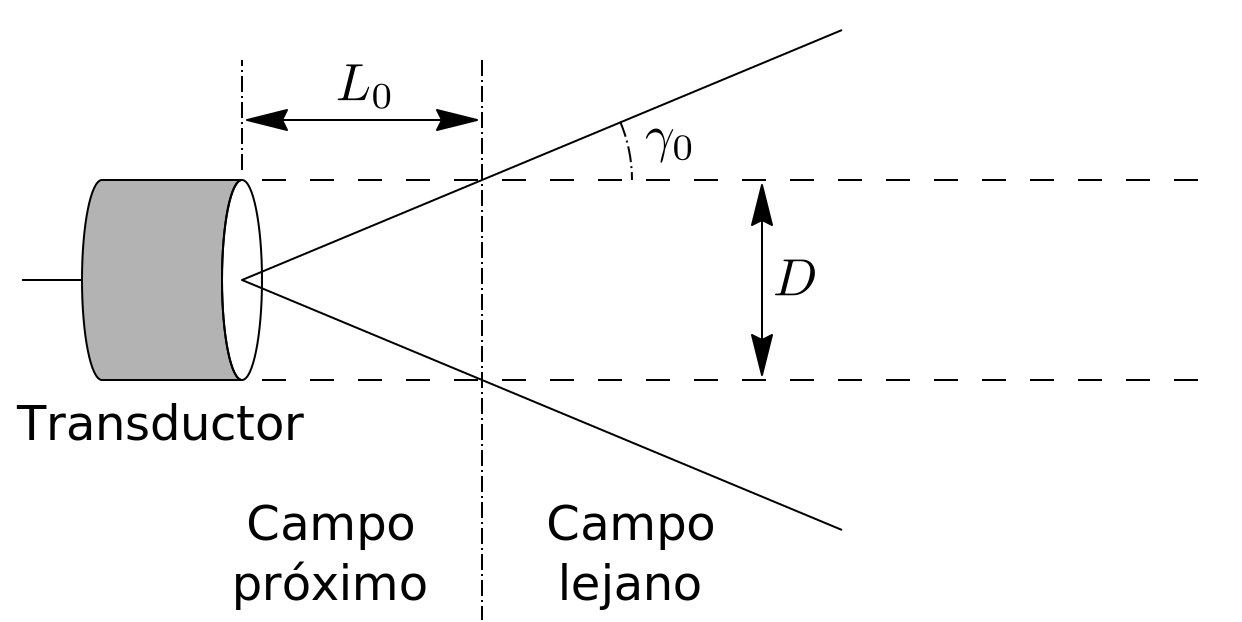
\includegraphics{gis-pfc-ch3-1.mps}
% 	\end{center}
% 	\caption{Campo generado por un transductor.}
% 	\label{fig:field}
% \end{figure}
% 
% \begin{figure}
% 	\begin{center}
% 		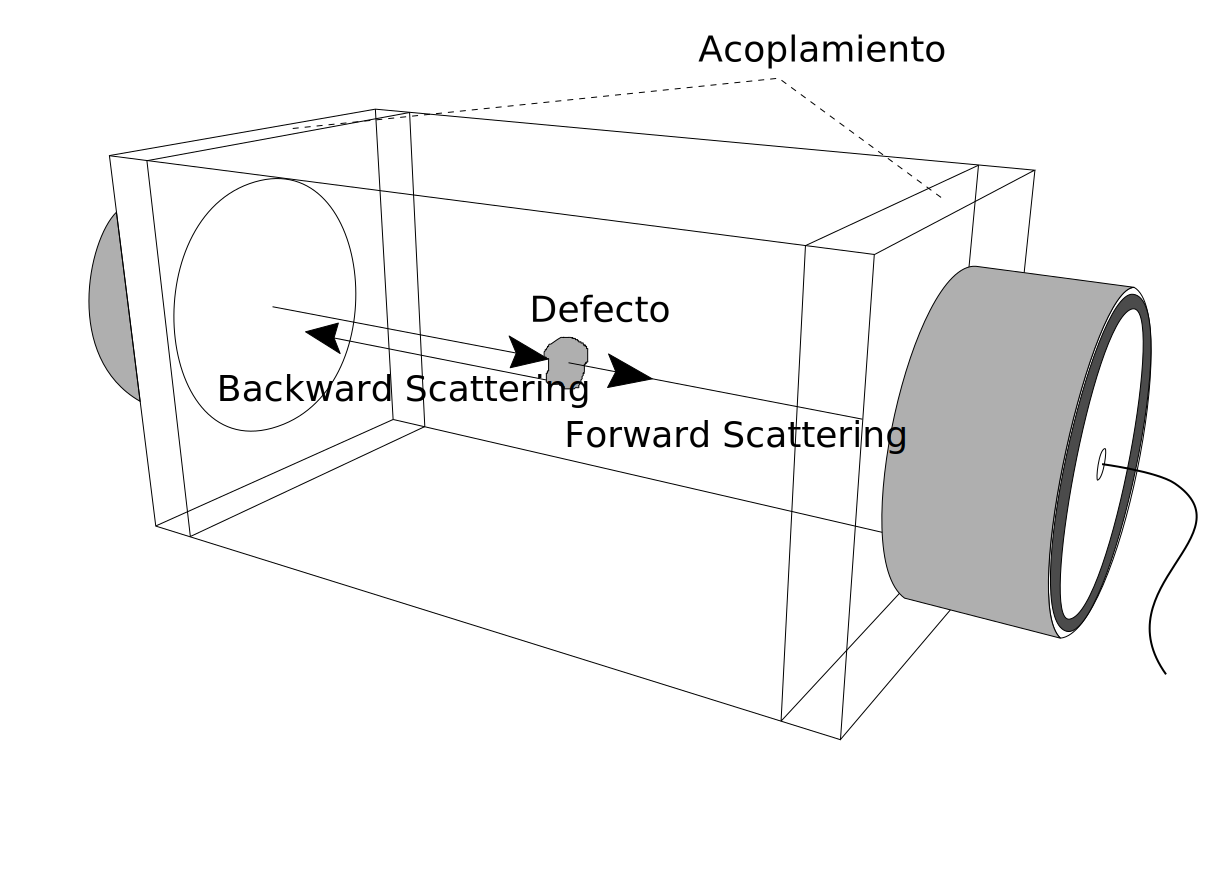
\includegraphics{gis-pfc-ch3-2.mps}
% 	\end{center}
% 	\caption{\textsc{endus} por transmisi�n.}
% 	\label{fig:transmission}
% \end{figure}
% 
% \begin{figure}
% 	\begin{center}
% 		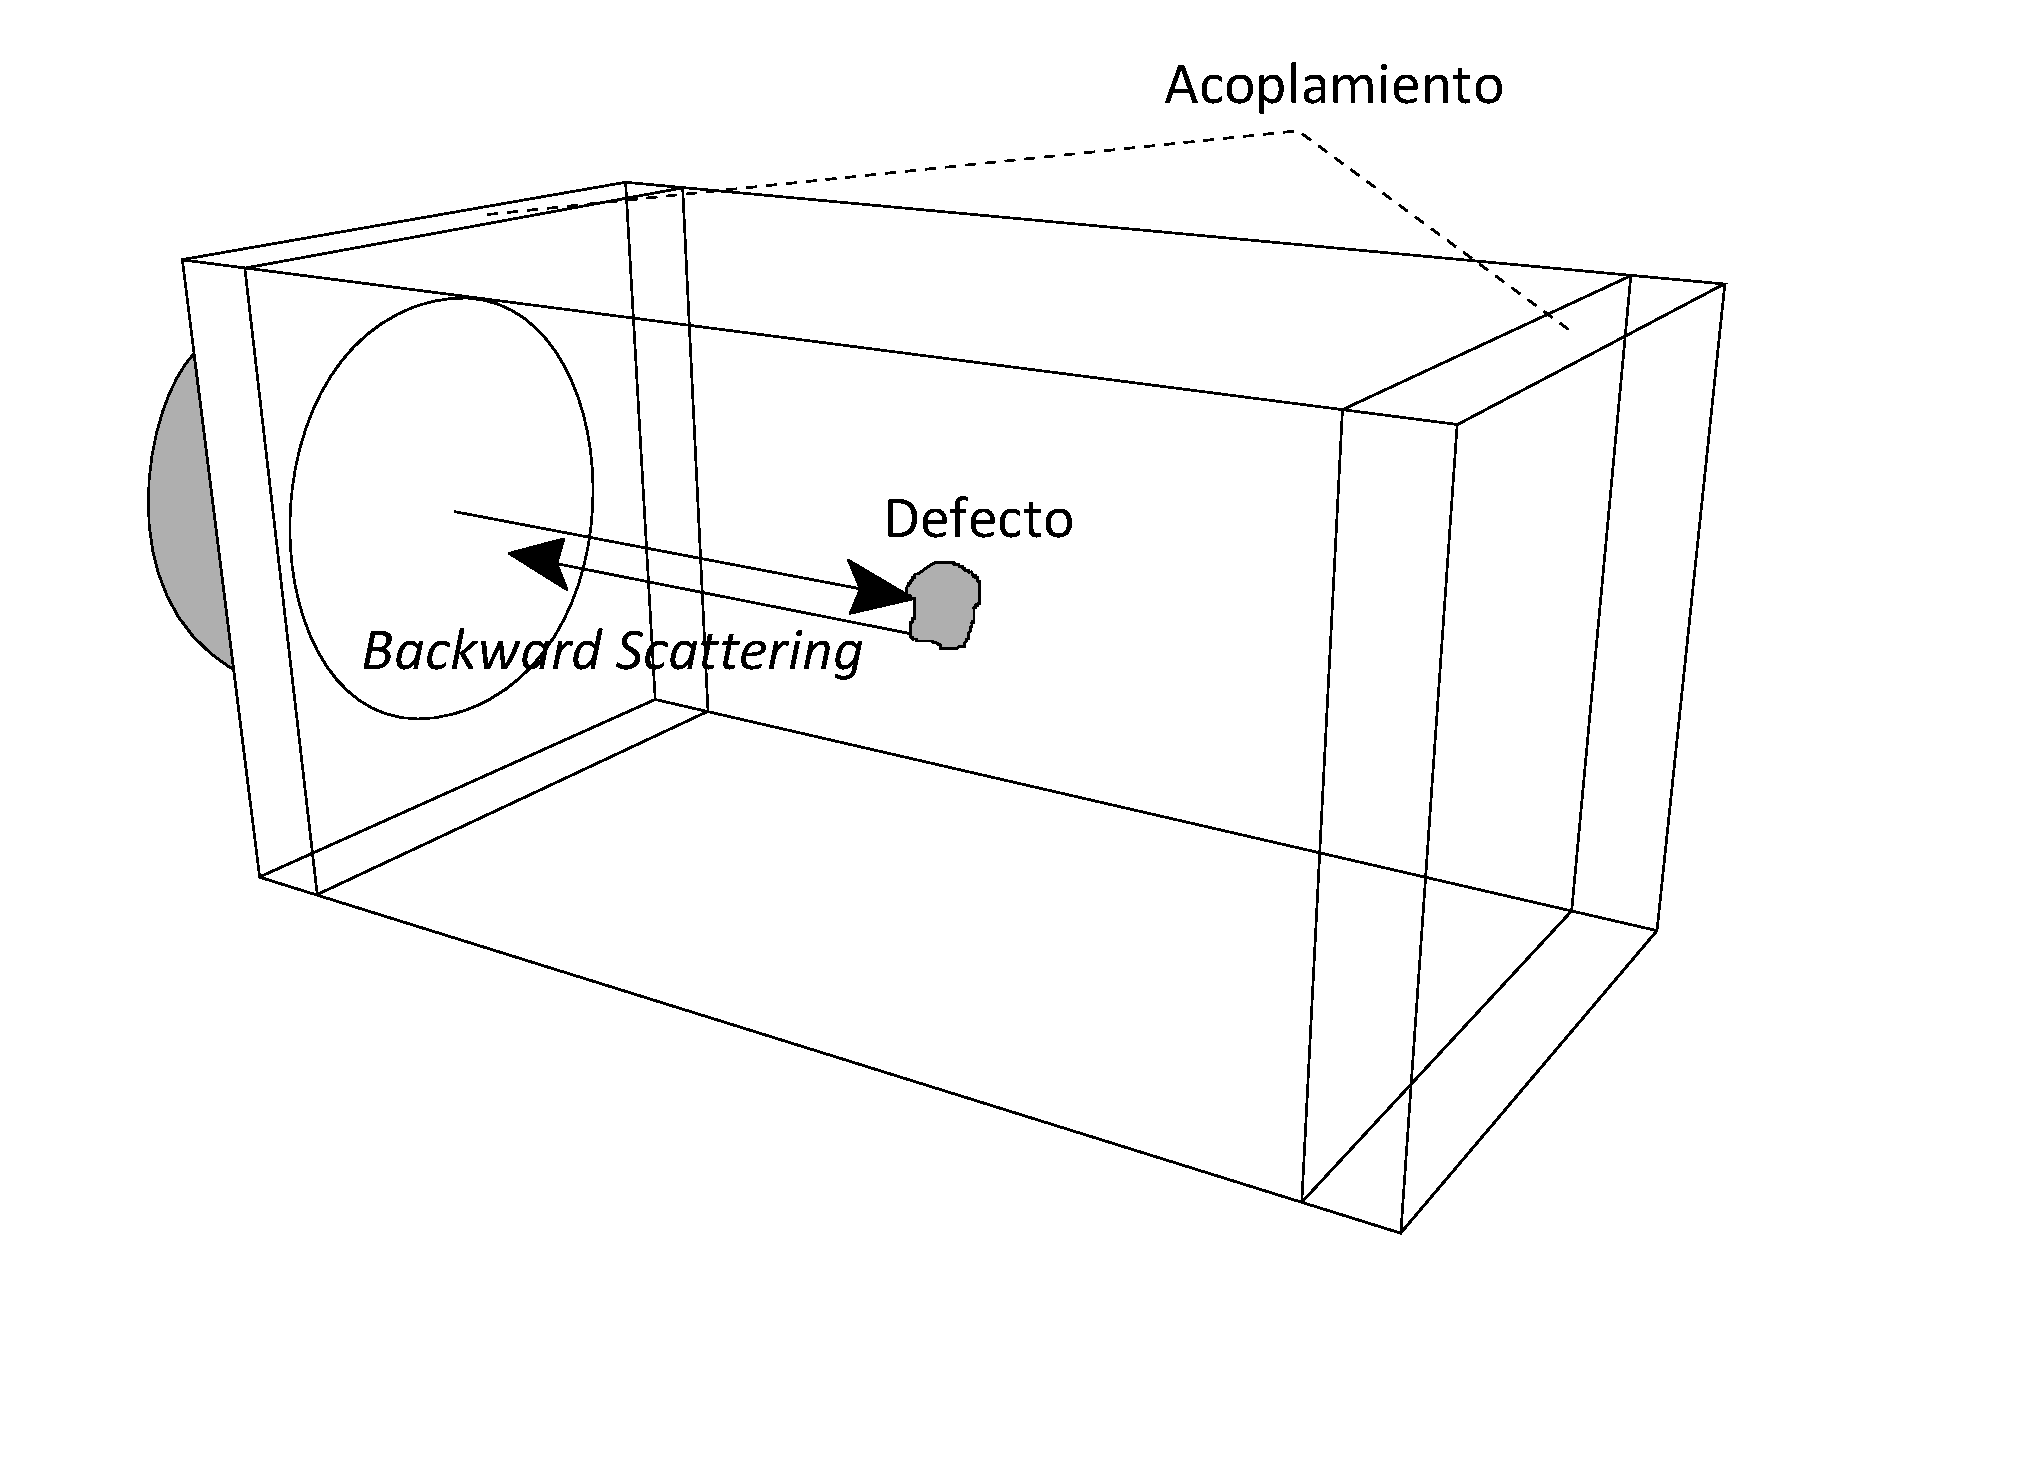
\includegraphics{gis-pfc-ch3-3.mps}
% 	\end{center}
% 	\caption{\textsc{endus} por pulso"=eco.}
% 	\label{fig:echo}
% \end{figure}
% 
% \begin{figure}
% 	\begin{center}
% 		\includegraphics{gis-pfc-ch3-4.mps}
% 	\end{center}
% 	\caption[Modelo de emisi�n"=transmisi�n]{Diagrama de bloques que muestra el modelo empleado para calcular la respuesta al impulso de emisi�n"=recepci�n.}
% 	\label{fig:model}
% \end{figure}
% 
% \begin{figure}
% 	\begin{center}
% 		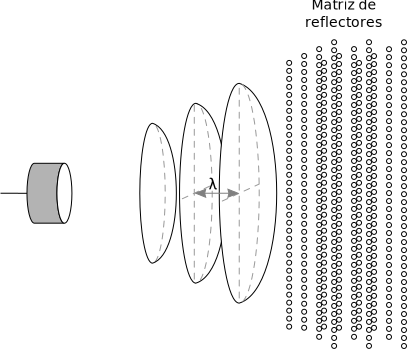
\includegraphics{gis-pfc-ch3-5.mps}
% 	\end{center}
% 	\caption{Modelo de matriz de peque�os reflectores.}
% 	\label{fig:matrix}
% \end{figure}
% 
% \begin{figure}
% 	\begin{center}
% 		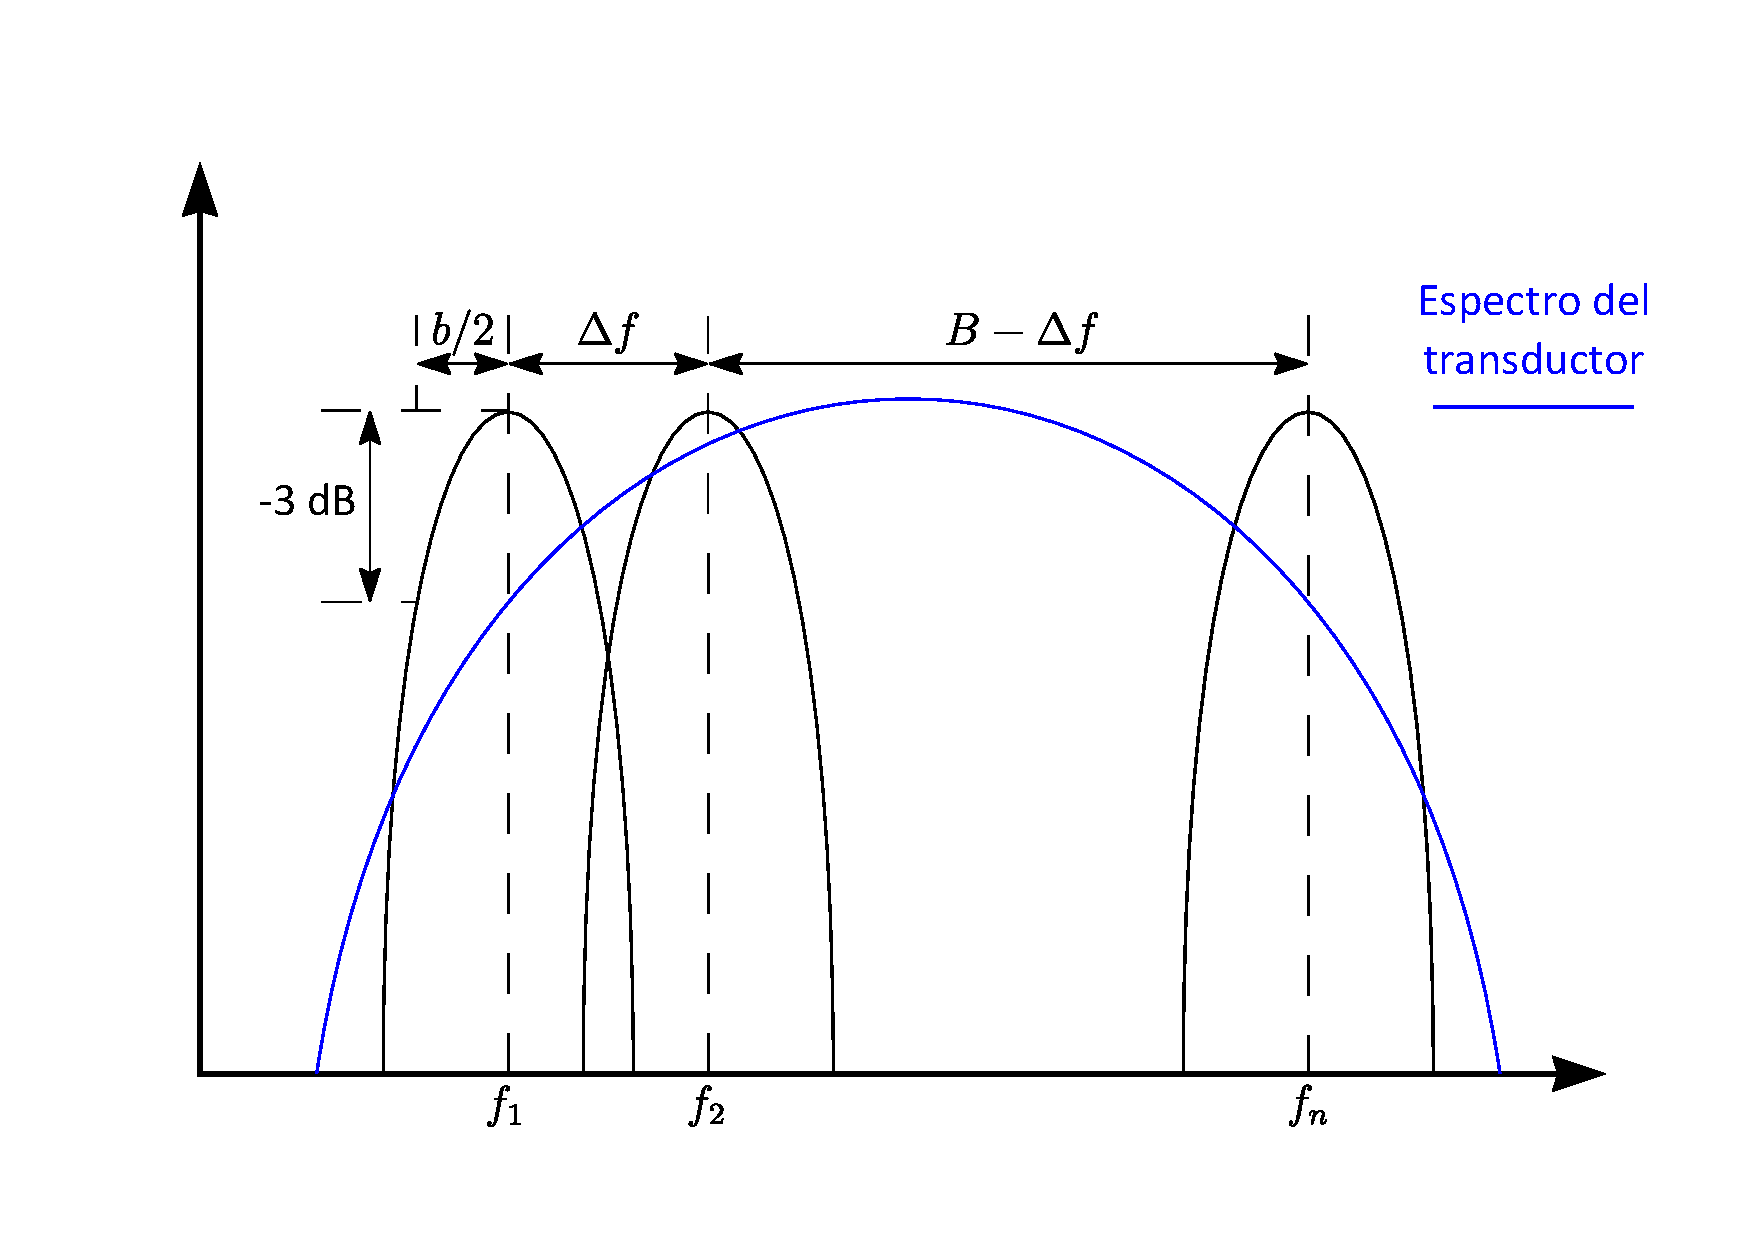
\includegraphics{gis-pfc-ch3-7.mps}
% 	\end{center}
% 	\caption[Par�metros del banco de filtros]{Representaci�n esquematizada en el que se identifican los par�metros de la \textsc{fft} y su relaci�n con respecto a la se�al.}
% 	\label{fig:filter}
% \end{figure}
% 
% \begin{figure}
% 	\begin{center}
% 		\includegraphics[angle=90]{gis-pfc-ch3-8.mps}
% 	\end{center}
% 	\caption{Circuito acondicionador de la secci�n de transmisi�n.}
% 	\label{fig:txaconditioner}
% \end{figure}
% 
% \begin{figure}
% 	\begin{center}
% 		\includegraphics{gis-pfc-ch3-9.mps}
% 	\end{center}
% 	\caption[Se�al a la salida del amplificador \textsc{ne5534}, $u(t)$]{Se�al generada por el acondicionador de transmisi�n medida a la salida del amplificador \textsc{ne5534}, $u(t)$.}
% 	\label{fig:txacvo}
% \end{figure}
% 
\begin{figure}
	\begin{center}
		\includegraphics{gis-pfc-ch3-10.mps}
	\end{center}
	\caption[Pulso ac�stico generado por el transductor]{Pulso ac�stico generado por el transductor cuando se alimenta con un pulso rectangular.}
	\label{fig:pulse}
\end{figure}
% 
% \newsavebox{\txbox}
% \sbox{\txbox}{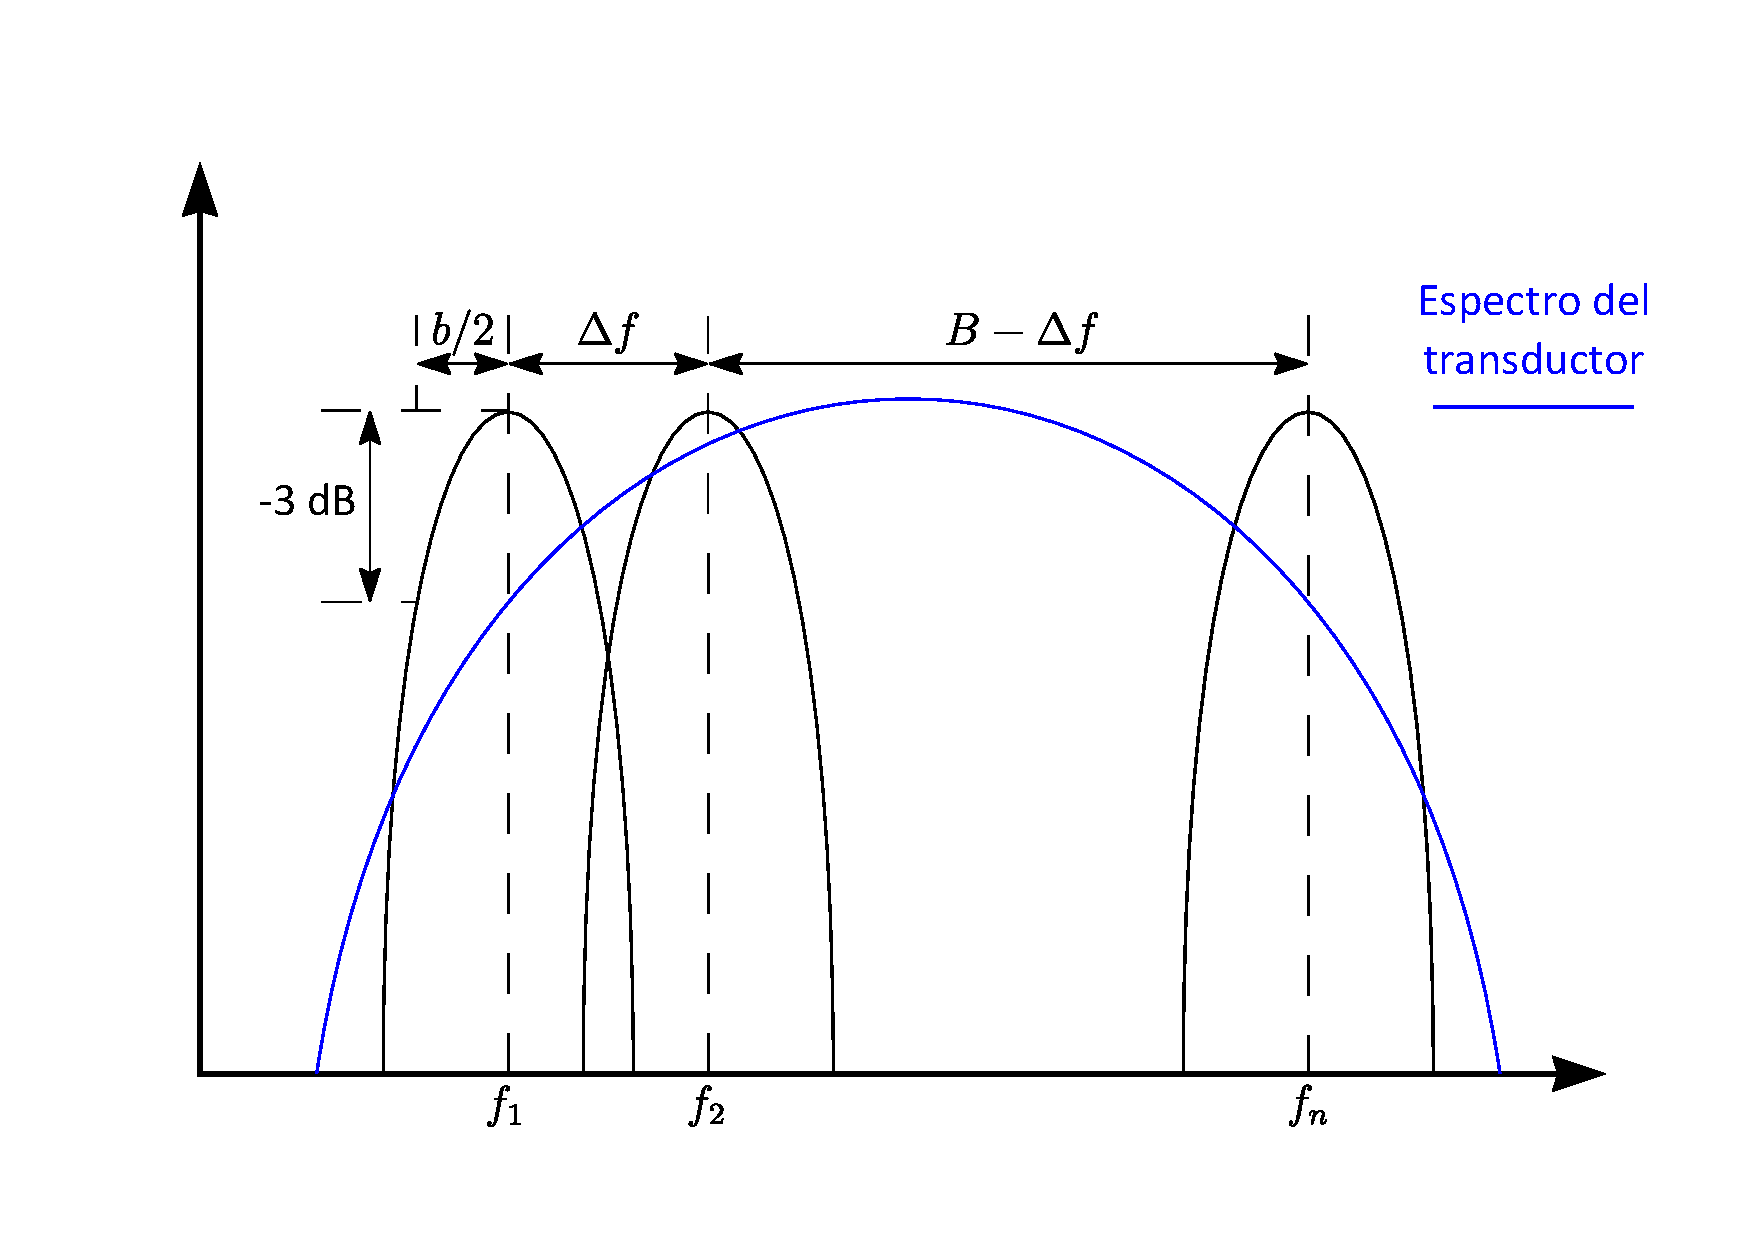
\includegraphics[draft=true]{gis-pfc-ch3-7.mps}}
% \newsavebox{\gxbox}
% \sbox{\gxbox}{\includegraphics[draft=true]{palm-trees-01.mps}}
% \newlength{\txwidth}
% \setlength{\txwidth}{4pt + \wd\txbox - \wd\gxbox}
% 
% \begin{figure}
% 	\begin{center}
% 		\hspace*{\txwidth}\includegraphics{palm-trees-01.mps}
% 	\end{center}
% 	\caption[Ejemplo de gr�fica]{Ejemplo de gr�fica con dimensiones de 120 mm de largo por 90 mm de alto.}
% 	\label{fig:palmone}
% \end{figure}

\end{document}
